
% v2-acmsmall-sample.tex, dated March 6 2012
% This is a sample file for ACM small trim journals
%
% Compilation using 'acmsmall.cls' - version 1.3 (March 2012), Aptara Inc.
% (c) 2010 Association for Computing Machinery (ACM)
%
% Questions/Suggestions/Feedback should be addressed to => "acmtexsupport@aptaracorp.com".
% Users can also go through the FAQs available on the journal's submission webpage.
%
% Steps to compile: latex, bibtex, latex latex
%
% For tracking purposes => this is v1.3 - March 2012
\documentclass[prodmode,acmtecs]{acmsmall} % Aptara syntax
\usepackage[spanish,polish]{babel}
\usepackage[T1]{fontenc}
\usepackage{fancyvrb}
\usepackage{graphicx,hyperref}
\newcommand\cutout[1]{}


\usepackage[table]{xcolor}
\usepackage[utf8]{inputenc}
\usepackage[parfill]{parskip}
\usepackage{tabulary}
\PassOptionsToPackage{hyphens}{url}
\usepackage{hyperref}    
\usepackage[capitalize]{cleveref}


% Metadata Information
% !!! TODO: SET THESE VALUES !!!
\acmVolume{0}
\acmNumber{0}
\acmArticle{CFP}
\acmYear{0}
\acmMonth{0}

\newcounter{colstart}
\setcounter{page}{4}

\RecustomVerbatimCommand{\VerbatimInput}{VerbatimInput}%
{
%fontsize=\footnotesize,
fontfamily=\rmdefault
}


\newcommand{\UnderscoreCommands}{%\do\verbatiminput%
\do\citeNP \do\citeA \do\citeANP \do\citeN \do\shortcite%
\do\shortciteNP \do\shortciteA \do\shortciteANP \do\shortciteN%
\do\citeyear \do\citeyearNP%
}

\usepackage[strings]{underscore}



% Document starts
\begin{document}


\setcounter{colstart}{\thepage}

\acmArticle{CFP}
\title{{\huge\sc SIGLOG Monthly 235}

 March 2023}
\author{DAVID PURSER\affil{University of Liverpool, UK}
\vspace*{-2.6cm}\begin{flushright}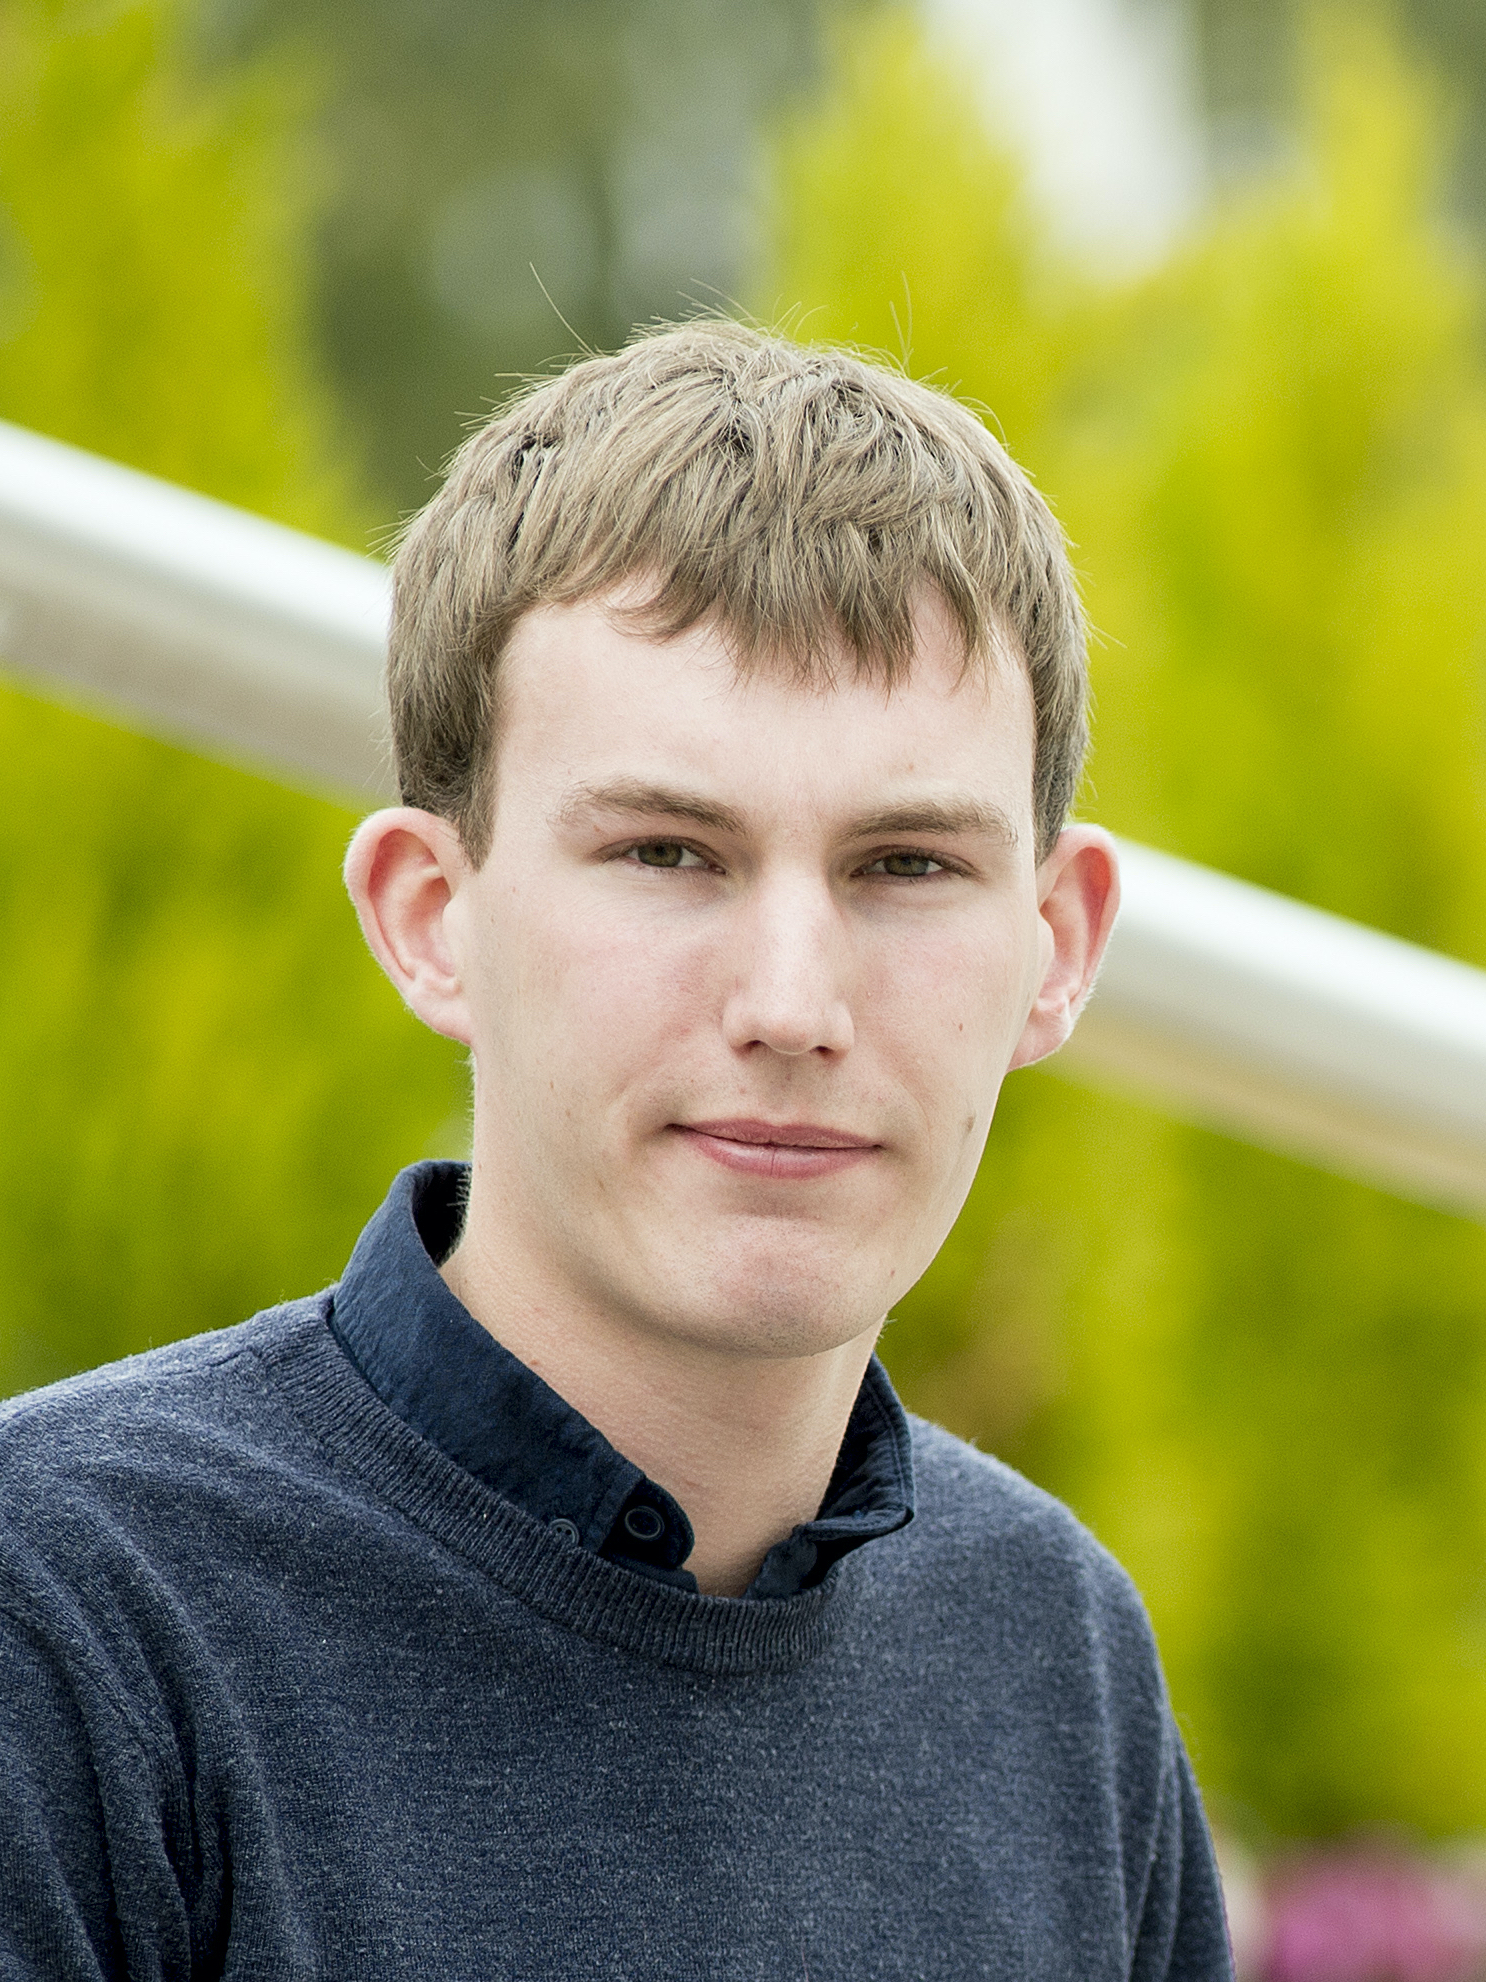
\includegraphics[width=30mm]{dp}\end{flushright}
}

\begin{abstract}
March 2023 edition of SIGLOG Monthly, featuring deadlines, calls and community announcements.
\end{abstract}


\maketitlee

\href{https://lics.siglog.org/newsletters/}{Past Issues}
 - 
\href{https://lics.siglog.org/newsletters/inst.html}{How to submit an announcement}
\section{Table of Content}\begin{itemize}\item DEADLINES (\cref{deadlines}) 
 
\item CALLS 
 
\begin{itemize}\item IWCS 2023 (CALL FOR PAPERS) (\cref{IWCS2023})
\item VCLA International Student Awards (CALL FOR NOMINATIONS) (\cref{VCLAInternationalStudentAwards})
\item InqBnB4 workshop (CALL FOR PAPERS) (\cref{InqBnB4workshop})
\item WiL 2023 (CALL FOR CONTRIBUTIONS) (\cref{WiL2023})
\item RSSRail 2023 (CALL FOR CONTRIBUTIONS) (\cref{RSSRail2023})
\item HOR 2023 (CALL FOR SUBMISSIONS) (\cref{HOR2023})
\item ACT 2023 (CALL FOR PAPERS) (\cref{ACT2023})
\item LORI 2023 (CALL FOR PAPERS) (\cref{LORI2023})
\item FSCD 2025 (CALL FOR LOCATION) (\cref{FSCD2025})
\end{itemize} 
\item JOB ANNOUNCEMENTS 
 
\begin{itemize}\item Assistant Professor with Tenure Track of Artificial Intelligence Ethics (\cref{AssistantProfessorwithTenureTrackofArtificialIntelligenceEthics})
\end{itemize} 
\end{itemize}\section{Deadlines}\label{deadlines}\rowcolors{1}{white}{gray!25}\begin{tabulary}{\linewidth}{LL}LOGIC COLLOQUIUM 2023:  & Mar 01, 2023 (Abstract), Mar 01, 2023 (Student Travel Grants deadline) \\
CAV 2023:  & Mar 01, 2023 (CAV AWARD Nomination deadline, Extended) \\
DEON 2023:  & Mar 01, 2023 (Abstract), Mar 31, 2023 (Paper) \\
Assistant Professor in Theoretical Computer Science in Amsterdam:  & Mar 14, 2023 (Deadline for application) \\
IWCS 2023:  & Mar 15, 2023 (Paper) \\
Assistant Professor with Tenure Track of Artificial Intelligence Ethics:  & Mar 16, 2023 (Application deadline) \\
ICDT 2024:  & Mar 20, 2023 (Cycle 1 Abstract), Mar 27, 2023 (Cycle 1 Full Submission due), Sep 13, 2023 (Cycle 2 Abstract), Sep 20, 2023 (Cycle 2 Full) \\
Faculty Positions at the University of Quebec in Montreal:  & Mar 31, 2023 (Application deadline) \\
VCLA International Student Awards:  & Mar 31, 2023 (Submission deadline) \\
CLAR 2023:  & Apr 10, 2023 (Submission deadline) \\
InqBnB4 workshop:  & Apr 14, 2023 (Submission deadline) \\
MARKTOBERDORF 2023:  & Apr 15, 2023 (Registration deadline) \\
FORMATS 2023:  & Apr 21, 2023 (Abstract), Apr 28, 2023 (Paper) \\
WiL 2023:  & Apr 23, 2023 (Abstract) \\
ICLP 2023:  & Apr 28, 2023 (non-regular paper) \\
RSSRail 2023:  & Apr 28, 2023 (Abstract  for all papers), Apr 28, 2023 (Abstract  for tutorials), May 05, 2023 (Full paper) \\
HOR 2023:  & May 02, 2023 (Submission deadline) \\
ACT 2023:  & May 03, 2023 (Submission Deadline) \\
GCM 2023:  & May 07, 2023 (Abstract), May 14, 2023 (Paper) \\
LORI 2023:  & May 15, 2023 (Paper  deadline) \\
FSCD 2025:  & May 27, 2023 (Deadline for location proposals) \\
\end{tabulary}
\section{IWCS 2023: 15th International Conference on Computational Semantics}\label{IWCS2023}  Université de Lorraine, Nancy, France\\ 
  20-23th June 2023   \\ 
  \href{http://iwcs2023.loria.fr/}{http://iwcs2023.loria.fr/}\\ 
CALL FOR PAPERS 

\begin{itemize}\item   IWCS is the biennial meeting of SIGSEM (\href{http://sigsem.org/}{http://sigsem.org/}), the ACL special interest group on semantics (\href{http://aclweb.org/}{http://aclweb.org/}); this year's edition is organized in person by the Loria (\href{https://www.loria.fr/fr/}{https://www.loria.fr/fr/}) and IDMC (\href{http://idmc.univ-lorraine.fr/}{http://idmc.univ-lorraine.fr/}) of the Université de Lorraine. 
 
  The aim of the IWCS conference is to bring together researchers interested in any aspects of the computation, annotation, extraction, representation and neuralisation of meaning in natural language, whether this is from a lexical or structural semantic perspective. IWCS embraces both symbolic and machine learning approaches to computational semantics, and everything in between. The conference and workshops will take place 20-23 June 2023. 
 
\item  TOPICS OF INTEREST 
 
  We invite paper submissions in all areas of computational semantics, in other words all computational aspects of meaning of natural language within written, spoken, signed, or multi-modal communication. 
 
  Presentations will be oral and posters. 
 
  Submissions are invited on these closely related areas, including the following: 
 
\begin{itemize}\item  design of meaning representations
\item  syntax-semantics interface
\item  representing and resolving semantic ambiguity
\item  shallow and deep semantic processing and reasoning
\item  hybrid symbolic and statistical approaches to semantics
\item  distributional semantics
\item  alternative approaches to compositional semantics
\item  inference methods for computational semantics
\item  recognising textual entailment
\item  learning by reading
\item  methodologies and practices for semantic annotation
\item  machine learning of semantic structures
\item  probabilistic computational semantics
\item  neural semantic parsing
\item  computational aspects of lexical semantics
\item  semantics and ontologies
\item  semantic web and natural language processing
\item  semantic aspects of language generation
\item  generating from meaning representations
\item  semantic relations in discourse and dialogue
\item  semantics and pragmatics of dialogue acts
\item  multimodal and grounded approaches to computing meaning
\item  semantics-pragmatics interface
\item  applications of computational semantics
\end{itemize} 
\item  SUBMISSION INFORMATION 
 
  Two types of submission are solicited: long papers and short papers. 
 
\begin{itemize}\item  Long papers should describe original research: max 8 pages excluding acknowledgements and references. 
\item  Short papers (typically system or project descriptions, or ongoing research): max 4 pages excluding acknowledgements and references.
\end{itemize} 
  Both types will be published in the conference proceedings and in the ACL Anthology. Accepted papers get an extra page in the camera-ready version. 
 
  See full call for formatting and submission instructions: \href{http://iwcs2023.loria.fr/call-for-papers/}{http://iwcs2023.loria.fr/call-for-papers/} 
 
\item  IMPORTANT DATES(anywhere on earth) 
 
\rowcolors{1}{white}{gray!25}\begin{tabulary}{\linewidth}{LL}Paper submission:  & Mar 15, 2023 \\
Decisions sent to authors:  & Apr 17, 2023 \\
Camera-ready papers due:  & May 15, 2023 \\
IWCS conference:  & Jun 20-23, 2023 \\
\end{tabulary}
 
\item   For questions, contact: iwcs2023-contact@univ-lorraine.fr 
 
\end{itemize}\section{VCLA International Student Awards}\label{VCLAInternationalStudentAwards}  \href{http://www.vcla.at/2023/01/call-for-nominations-vcla-international-student-awards/}{http://www.vcla.at/2023/01/call-for-nominations-vcla-international-student-awards/}\\ 
  \href{https://logic-cs.at/vcla-international-student-awards-2023/}{https://logic-cs.at/vcla-international-student-awards-2023/}\\ 
CALL FOR NOMINATIONS 

\begin{itemize}\item   The Vienna Center for Logic and Algorithms of TU Wien calls for the nomination of authors of outstanding theses and scientific works in the field of Logic and Computer Science, in the following two categories: 
 
\begin{itemize}\item  Outstanding Master Thesis Award*
\item  Outstanding Undergraduate Thesis Award (Bachelor thesis or equivalent, 1st cycle of the Bologna process)*
\end{itemize} 
  The degree must have been awarded between January 1st, 2021 and December 31st, 2022 (inclusive). 
 
\item  The main areas of interest are: 
 
\begin{itemize}\item  Computational Logic, covering theoretical and mathematical foundations such as proof theory, model theory, computability theory, Boolean satisfiability (SAT), QBF, constraint satisfaction, satisfiability modulo theories, automated deduction (resolution, refutation, theorem proving), non-classical logics (substructural logics, multi-valued logics, deontic logics, modal and temporal logics).
\item  Algorithms and Computational Complexity, including design and analysis of discrete algorithms, complexity analysis, algorithmic lower bounds, parameterized and exact algorithms, decomposition methods, approximation algorithms, randomized algorithms, algorithm engineering, as well as algorithmic game theory, computational social choice, parallel algorithms, graph drawing algorithms, and distributed algorithms.
\item  Databases and Artificial Intelligence, concerned with logical methods for modeling, storing, and drawing inferences from data and knowledge. This includes subjects like query languages based on logical concepts (Datalog, variants of SQL, XML, and SPARQL), novel database-theoretical methods (schema mappings, information extraction and integration), logic programming, knowledge representation and reasoning (ontologies, answer-set programming, belief change, inconsistency handling, argumentation, planning).
\item  Verification, concerned with logical methods and automated tools for reasoning about the behavior and correctness of complex state-based systems such as software and hardware designs as well as hybrid systems. This ranges from model checking, program analysis and abstraction to new interdisciplinary areas such as fault localization, program repair, program synthesis, and the analysis of biological systems.
\end{itemize} 
\item  AWARDS 
 
\begin{itemize}\item  The Outstanding Master Thesis Award: 1200 EUR.
\item  The Outstanding Undergraduate Thesis Award: 800 EUR.
\end{itemize} 
  The winners will be invited to present their work at an award ceremony in Vienna, if the situation allows. 
 
\item  ELIGIBILITY 
 
\begin{itemize}\item  The degree must have been awarded between January 1st, 2021 and December 31st, 2022 (inclusive).
\item  Students who obtained their degree at TU Wien are not eligible.
\end{itemize} 
\item  NOMINATION REQUIREMENTS 
 
  Nominations must include: 
 
\begin{itemize}\item  A cover page that contains the name and contact details of the nominated person, the title of the work for which the person is being nominated, award category, the date on which the degree was awarded, and the name of the university.
\item  An English summary of the thesis of maximum 3 pages, excluding references (A4 or letter page size, 11pt font min). The summary must clearly state the main contribution of the work, its novelty, and its relevance to some of the aforementioned areas of interest.
\item  The CV of the nominated person, including publication list (if applicable).
\item  An endorsement letter from a supervisor or another proposing person. The letter must clearly state the independent and novel contribution of the student, and why the proposer believes the student deserves the award. The endorsement letter may be provided after the submission deadline, and emailed directly to award (AT) logic-cs.at.
\item  The full thesis.
\end{itemize} 
  All documents should be in English, with the exception of the thesis. In case the thesis is in a different language, it must be accompanied by a research report in English of at least 10 pages that should be sufficient for the committee to evaluate the merit and quality of the submitted work. 
 
\item  INSTRUCTIONS 
 
  Instructions for submitting self-nominations 
 
\begin{itemize}\item  Nominations should be submitted electronically by the applicants using the following link to EasyChair: \href{https://easychair.org/conferences/?conf=vclaawards2023}{https://easychair.org/conferences/?conf=vclaawards2023}.
\item  Submissions consist of two pdf files. The first is a single pdf file containing all documents for the nomination except the full thesis; the documents should appear in the order they are listed above. The second pdf file is the full thesis.
\item  The endorsement letter may optionally be sent by email by the endorser and omitted from the Easychair submission. In this case, please email the letter as a pdf file, including the name of the nominated person in the subject, to award (AT) logic-cs DOT at.
\item  The submission must be accompanied by a plain text electronic abstract of the thesis of at most 400 words, and three keywords.
\item  The nominated student must be listed as the only author in the submission form.
\end{itemize} 
\item  IMPORTANT DATES (AoE) 
 
\rowcolors{1}{white}{gray!25}\begin{tabulary}{\linewidth}{LL}Submission deadline:  & Mar 31, 2023 \\
Notification of decision:  & After Jun 30, 2023 \\
\end{tabulary}
 
\item  CONTACT 
 
  Please send all inquiries to award@logic-cs.at. 
 
\end{itemize}\section{InqBnB4 workshop: Inquisitiveness Below and Beyond the Sentence Boundary}\label{InqBnB4workshop}  Nancy (France), 20 June 2023, hosted by IWCS 2023\\ 
  \href{https://iwcs2023.loria.fr/inqbnb4-inquisitiveness-below-and-beyond-the-sentence-boundary/}{https://iwcs2023.loria.fr/inqbnb4-inquisitiveness-below-and-beyond-the-sentence-boundary/}\\ 
CALL FOR PAPERS 

\begin{itemize}\item  InqBnB is a workshop series bringing together researchers interested in the semantics and pragmatics of interrogatives (questions or embedded interrogative clauses). This series was originally organized by the Inquisitive Semantics Group of the Institute for Logic, Language and Computation (ILLC) from the University of Amsterdam. As such, the focus point mainly revolves around analyses using or related to inquisitive semantics. 
 
  After three successful editions in the Netherlands, we hope to open the inquisitive community to a wider audience. The 4th edition is planned on 20 June 2023, just before IWCS 2023 (Internation Conference on Computational Semantics). As invited speakers we are welcoming Wataru Uegaki (University of Edinburgh) and one other to be announced. 
 
  InqBnB4 invites submissions on original and unpublished research focussed on the properties of inquisitive content. We are mainly interested in theoretical questions, formal models and empirical work. But we are also welcoming papers based on statistical or neural models, provided their main goal is to bring new insights regarding inquisitiveness. 
 
  Here are some examples of questions of interest:  
 
\begin{itemize}\item  Which operators (connectives, quantifiers, modals, conditionals) generate inquisitiveness? 
\item  How do these operators project the inquisitive content of their arguments? e.g. what triggers maximality, exhaustivity or uniqueness of readings? 
\item  How does inquisitive content interact with informative content in compositional semantics? e.g. how do interrogative words interact with negative polarity items, free choice items, indefinites or plurality? 
\item  How do conventions of use interact with inquisitive content? e.g. how can non-answering responses (e.g. clarification questions) be handled? 
\item  In which ways is pragmatics sensitive to inquisitive content? e.g. how does answer bias and ignorance inferences arise? 
\item  What kind of discourse anaphora are licensed by inquisitive expressions? e.g. does dynamic inquisitive semantics manage to correctly derive donkey anaphora?
\end{itemize} 
\item  SUBMISSION: Submission link on SoftConf: \href{https://softconf.com/iwcs2023/inqbnb4/}{https://softconf.com/iwcs2023/inqbnb4/} 
 
  Sumitted papers must not exceed eight (8) pages (not counting acknowledgement, references and appendices). Accepted papers get an extra page in the camera-ready version. Submitted papers should be formatted following the common two-column structure as used by ACL. Please use the specific style-files or the Overleaf template for IWCS 2023, taken from ACL 2021. Initial submissions should be fully anonymous to ensure double-blind reviewing. The proceedings will be published in the ACL anthology. 
 
\item  IMPORTANT DATES:  
 
\rowcolors{1}{white}{gray!25}\begin{tabulary}{\linewidth}{LL}Submission deadline:  & Apr 14, 2023 \\
Author notification:  & May 12, 2023 \\
Camera ready:  & Jun 09, 2023 \\
Workshop day:  & Jun 20, 2023 \\
\end{tabulary}
 
\end{itemize}\section{WiL 2023: 7th Women in Logic Workshop}\label{WiL2023}  July 1, 2023\\ 
  Co-located with FSCD 2023\\ 
  \href{https://sites.google.com/view/wil2023/home}{https://sites.google.com/view/wil2023/home}\\ 
CALL FOR CONTRIBUTIONS 

\begin{itemize}\item  Women in Logic 2023 is a satellite event of the  8th International Conference on Formal Structures for Computation and Deduction (FSCD 2023) to be held in Rome, Italy, from July 1 to July 6, 2023. 
 
  The Women in Logic workshop (WiL) provides an opportunity to increase awareness of the valuable contributions made by women in the area of logic in computer science. Its main purpose is to promote the excellent research done by women, with the ultimate goal of increasing their visibility and representation in the community. Our aim is to: 
 
\begin{itemize}\item  provide a platform for female researchers to share their work and achievements;
\item  increase the feelings of community and belonging, especially among junior faculty, post-docs and students through positive interactions with peers and more established faculty;
\item  establish new connections and collaborations;
\item  foster a welcoming culture of mutual support and growth within the logic research community.
\end{itemize} 
  We believe these aspects will benefit women working in logic and computer science, particularly early-career researchers. 
 
  Previous versions of Women in Logic (Reykjavík 2017, Oxford 2018, Vancouver 2019, Paris 2020, Rome 2021, and Haifa 2022) were very successful in showcasing women's work and as catalysts for a recognition of the need for change in the community. 
 
\item  Topics of interest include but are not limited to: automata theory, automated deduction, categorical models and logics, concurrency and distributed computation, constraint programming, constructive mathematics, database theory, decision procedures, description logics, domain theory, finite model theory, formal aspects of program analysis, formal methods, foundations of computability, games and logic, higher-order logic, lambda and combinatory calculi, linear logic, logic in artificial intelligence, logic programming, logical aspects of bioinformatics, logical aspects of computational complexity, logical aspects of quantum computation, logical frameworks, logics of programs, modal and temporal logics, model checking, probabilistic systems, process calculi, programming language semantics, proof theory, real-time systems, reasoning about security and privacy, rewriting, type systems and type theory, and verification. 
 
\item  INVITED SPEAKERS 
 
\begin{itemize}\item  Marie Kerjean (LIPN, Institut Galilée)
\item  TBA
\end{itemize} 
\item  IMPORTANT DATES 
 
\rowcolors{1}{white}{gray!25}\begin{tabulary}{\linewidth}{LL}Abstract submission:  & Apr 23, 2023 \\
Notification:  & May 15, 2023 \\
Contribution for Informal Proceedings:  & Jun 25, 2023 \\
Workshop:  & Jul 01, 2023 \\
\end{tabulary}
 
\item  SUBMISSIONS 
 
  Abstracts should be written in English (1-2 pages), and prepared using the Easychair style (\href{https://easychair.org/publications/for_authors}{https://easychair.org/publications/for\_authors}). The abstracts should be uploaded to the WiL 2023 Easychair page \href{https://easychair.org/my/conference?conf=wil2023}{https://easychair.org/my/conference?conf=wil2023} as a PDF file before the submission deadline on April 23, 2023, anywhere on Earth. 
 
\end{itemize}\section{RSSRail 2023: International conference on reliability, safety and security of railway systems - modelling, analysis, verification and certification}\label{RSSRail2023}  October 10-12, 2023, Berlin, Germany\\ 
  \href{https://rssr2023.ebuef.de/}{https://rssr2023.ebuef.de/}\\ 
CALL FOR CONTRIBUTIONS 

\begin{itemize}\item  The railway industry faces increasing pressure to improve system safety, to decrease production costs and time to market, to reduce carbon emissions and running costs, and to increase the capacity of the railway. Railway systems are now being integrated into larger multi-transport networks. Such systems require an even higher degree of automation at all levels of operation. These trends dramatically increase the complexity of railway applications and pose new challenges in developing novel methods of modelling, analysis, verification and validation to ensure their reliability, safety and security, as well as in supporting novel mechanisms and procedures to help make the case that development processes meet the mandated standards. 
 
  This conference will bring together researchers and developers working on railway system reliability, security and safety to discuss how all of these requirements can be met in an integrated way. It is also vital to ensure that advances in research (in both academia and industry) are driven by the real industrial needs. This will help ensure that such advances are followed by effective industrial deployment. Another particularly important objective is to integrate advances in research into the current development processes, and make them usable and scalable. Finally, a key goal is to develop advanced methods and tools that can ensure that the systems meet the requirements imposed by the regulatory standards and help in building the supportive arguments. This will be a working conference in which research challenges and progress will be discussed and evaluated by both researchers and engineers, focusing on their potential to be deployed in industrial settings. 
 
\item  TOPICS OF PARTICULAR INTEREST: 
 
\begin{itemize}\item  Safety in development processes and safety management
\item  Combined approaches to safety and security
\item  System and software safety analysis
\item  Formal modelling and verification techniques
\item  System reliability
\item  Validation according to the standards
\item  Safety and security argumentation
\item  Fault and intrusion modelling and analysis
\item  Evaluation of system capacity, energy consumption, cost and their interplay
\item  Tool and model integration, tool chain
\item  Domain-specific languages and modelling frameworks
\item  Model reuse for reliability, safety and security
\item  Modelling for maintenance strategy engineering.
\end{itemize} 
\item  PRESENTATIONS 
 
  The conference offers different options for presenting research: 
 
\begin{itemize}\item  Regular conference papers of 16 pages
\item  Industrial conference papers of 10 pages, providing real-life feedback
\item  Student conference papers of 10 pages, showcasing novel ideas and early research results
\item  Poster presentation, not to be accompanied by a full paper, however the abstract will be published on the website
\item  Tutorials to be offered in the first day (in total 4 tutorials a 90 minute in two parallel sessions).
\end{itemize} 
\item  IMPORTANT DATES: 
 
\rowcolors{1}{white}{gray!25}\begin{tabulary}{\linewidth}{LL}Abstract submission for all papers:  & Apr 28, 2023 \\
Abstract submission for tutorials:  & Apr 28, 2023 \\
Full paper submission:  & May 05, 2023 \\
Notification:  & Jun 16, 2023 \\
Camera-ready papers submitted:  & Jul 14, 2023 \\
Abstract submission for posters:  & Jul 14, 2023 \\
\end{tabulary}
 
\item  PROCEEDINGS 
 
  The conference proceedings will be published by Springer in the LNCS series. The conference submission will be via \href{https://www.tu.berlin/bbi/rssr2023}{https://www.tu.berlin/bbi/rssr2023} Submissions must be formatted in the Springer LNCS format, see \href{https://www.springer.com/gp/computer-science/lncs/conference-proceedings-guidelines}{https://www.springer.com/gp/computer-science/lncs/conference-proceedings-guidelines}. 
 
\end{itemize}\section{HOR 2023: 11th International Workshop on Higher-Order Rewriting}\label{HOR2023}   4 July 2023\\ 
   Rome, Italy\\ 
   \href{https://hor2023.github.io/}{https://hor2023.github.io/}\\ 
   HOR 2023 is affiliated with FSCD 2023\\ 
   \href{https://easyconferences.eu/fscd2023/}{https://easyconferences.eu/fscd2023/}\\ 
CALL FOR SUBMISSIONS 

\begin{itemize}\item  OVERVIEW 
 
  HOR is a forum to present work concerning all aspects of higher-order rewriting. 
 
  HOR aims to provide an informal and friendly setting to discuss recent work and work in progress concerning higher-order rewriting, broadly construed. This includes rewriting systems that have functional variables or bound variables, the lambda-calculus and combinatory logic being paradigmatic examples. 
 
\item  TOPICS 
 
  The following is a non-exhaustive list of topics for the workshop: 
 
\begin{itemize}\item  Applications: proof checking, theorem proving, generic programming, declarative programming, program transformation, automated termination/confluence/equivalence analysis tools.
\item  Foundations: pattern matching, unification, strategies, narrowing, termination, syntactic properties, type theory, complexity of derivations.
\item  Frameworks: term rewriting, conditional rewriting, graph rewriting, net rewriting, comparisons of different frameworks.
\item  Implementation: explicit substitution, rewriting tools, compilation techniques.
\item  Semantics: semantics of higher-order rewriting, categorical rewriting, higher-order abstract syntax, games and rewriting.
\end{itemize} 
\item  SUBMISSION GUIDELINES  
 
  To give a presentation at the workshop, please submit an extended abstract (between 2 to 5 pages) via Easychair: \href{https://easychair.org/conferences/?conf=hor2023}{https://easychair.org/conferences/?conf=hor2023}  
 
  Please use LaTeX and the Easychair style to prepare your submission: \href{https://easychair.org/publications/easychair.zip}{https://easychair.org/publications/easychair.zip} 
 
  HOR is a platform for discussing open questions, ongoing research, and new perspectives, as well as new results. Extended abstracts describing work in progress, preliminary results, research projects, or problems in higher-order rewriting are very welcome. Specifically, short versions of recently published papers are welcome, and submission to HOR does not preclude formal publication at other venues. 
 
  The workshop has informal electronic proceedings that will be made available on the workshop website. 
 
\item  IMPORTANT DATES 
 
\rowcolors{1}{white}{gray!25}\begin{tabulary}{\linewidth}{LL}Submission deadline:  & May 02, 2023 \\
Notification:  & May 29, 2023 \\
Final version:  & Jun 12, 2023 \\
\end{tabulary}
 
\end{itemize}\section{ACT 2023: 6th Annual International Conference on Applied Category Theory}\label{ACT2023}  July 31 – August 4, 2023\\ 
  \href{https://act2023.github.io/}{https://act2023.github.io/}\\ 
CALL FOR PAPERS 

\begin{itemize}\item  The Sixth International Conference on Applied Category Theory will take place at the University of Maryland from 31 July to 4 August 2023, preceded by the Adjoint School 2023 from 24 to 28 July. This conference follows previous events at Strathclyde (UK), Cambridge (UK), Cambridge (MA), Oxford (UK) and Leiden (NL).  
 
  Applied category theory is important to a growing community of researchers who study computer science, logic, engineering, physics, biology, chemistry, social science, systems, linguistics and other subjects using category-theoretic tools.  The background and experience of our members is as varied as the systems being studied. The goal of the Applied Category Theory conference series is to bring researchers together, strengthen the applied category theory community, disseminate the latest results, and facilitate further development of the field. 
 
\item  SUBMISSIONS  
 
  We accept submissions in English of original research papers, talks about work accepted/submitted/published elsewhere, and demonstrations of relevant software. Accepted original research papers will be published in a proceedings volume. The conference will include an industry showcase event and community meeting. We particularly encourage people from underrepresented groups to submit their work and the organizers are committed to non-discrimination, equity, and inclusion.  
 
  Original research papers intended for conference proceedings should present original, high-quality work in the style of a computer science conference paper (up to 12 pages, not counting the bibliography; more detailed parts of proofs may be included in an appendix for the convenience of the reviewers). Please use the EPTCS style files available at <\href{http://style.eptcs.org}{http://style.eptcs.org}>. Such submissions should not be an abridged version of an existing journal article although pre-submission arXiv preprints are permitted. These submissions will be adjudicated for both a talk and publication in the conference proceedings.  
 
\item  IMPORTANT DATES (AoE) 
 
\rowcolors{1}{white}{gray!25}\begin{tabulary}{\linewidth}{LL}Submission Deadline:  & May 03, 2023 \\
Author Notification:  & Jun 07, 2023 \\
Camera-ready version due:  & Jun 27, 2023 \\
Conference begins:  & Jul 31, 2023 \\
\end{tabulary}
 
\end{itemize}\section{LORI 2023: International Conference on Logic, Rationality and Interaction}\label{LORI2023}  26-29 October 2023, Shandong, China\\ 
CALL FOR PAPERS 

\begin{itemize}\item  The International Conference on Logic, Rationality and Interaction (LORI) conference series aims at bringing together researchers working on a wide variety of logic-related topics that concern the understanding of rationality and interaction. The series aims at fostering a view of Logic as an interdisciplinary endeavour, and supports the creation of an East-Asian community of interdisciplinary researchers. 
 
  We invite submission of contributed papers on any of the broad themes of LORI series; specific topics of interest include, but are not limited to, formal approaches to 
 
\begin{itemize}\item  agency
\item  argumentation and agreement
\item  belief representation
\item  probability and uncertainty
\item  belief revision and belief merging
\item  knowledge and action
\item  dynamics of informational attitudes
\item  intentions, plans, and goals
\item  decision making and planning
\item  preference and utility
\item  cooperation
\item  strategic reasoning and game theory
\item  epistemology
\item  social choice
\item  social interaction
\item  speech acts
\item  knowledge representation
\item  norms and normative systems
\item  natural language
\item  rationality
\item  philosophical logic
\end{itemize} 
\item  Submitted papers should be at most 12 pages long, with one additional page for references, in PDF format following the Springer LNCS style, submitted via EasyChair (\href{https://easychair.org/conferences/?conf=lori9}{https://easychair.org/conferences/?conf=lori9}). Accepted papers will be collected as a volume in the FoLLI Series on Logic, Language and Information, and authors may be later invited to submit extended versions of their papers in a special issue of a prestigious journal. 
 
Paper submission deadline: May 15, 2023 
 
  For detailed conference information and registration, please visit golori.org/lori2023/  
 
\end{itemize}\section{FSCD 2025: International Conference on Formal Structures for Computation and Deduction}\label{FSCD2025}CALL FOR LOCATION 

\begin{itemize}\item  The FSCD conference covers all aspects of Formal Structures for Computation and Deduction from theoretical foundations to applications.  The annual FSCD conference comprises the main conference and a considerable number of affiliated workshops (expectedly, more than ten). We invite proposals for locations to host the 10th FSCD International Conference to be held during the summer of 2025.  
 
Deadline for location proposals: May 27, 2023 
 
  Proposals should be sent to the FSCD Steering Committee Chair (see contact information below). We encourage proposers to register their intention informally as soon as possible. 
 
  Previous (and upcoming) FSCD meetings include: 
 
\begin{itemize}\item  FSCD 2016 in Porto (Portugal);
\item  FSCD 2017 in Oxford (UK) co-located with ICFP 2017;
\item  FSCD 2018 in Oxford (UK) as part of FLoC 2018;
\item  FSCD 2019 in Dortmund (Germany);
\item  FSCD 2020 in Paris (France) co-located with IJCAR 2020;
\item  FSCD 2021 in Buenos Aires (Argentina);
\item  FSCD 2022 in Haifa (Israel) as part of FLOC2022;
\item  FSCD 2023 in Rome (Italy) co-located with CADE 2023;
\item  FSCD 2024 in Tallinn (Estonia).
\end{itemize} 
  Selected proposals are to be presented at the business meeting of FSCD 2023 taking place in Rome in July 2023.  The final decision about hosting and organising of FSCD 2025 will be taken by the SC after an advisory vote of the members of the community in attendance at the business meeting. 
 
\item  Proposals should address the following points: 
 
\begin{itemize}\item  FSCD Conference Chair (complete name and current position), host institution, FSCD Local Committee (complete names and current positions), availability of student-volunteers.
\item  National, regional, and local government and industry support, both organizational and financial.
\item  Accessibility to the location (i.e., transportation) and attractiveness of the proposed site. Accessibility can include both information about local transportation and travel information to the location (flight and/or train connections), as well as estimated costs.
\item  Proposed dates, including allowing 2-3 days before and/or after the main conference for affiliated workshops. (Please also take into consideration holidays or local events during the period).
\item  Estimated costs of registration for the conference and workshops, both for regular and student participants.
\item  Conference and exhibit facilities for the anticipated number of registrants (including all workshop participants, typically around 200). For example: number, capacity and audiovisual equipment of meeting rooms; a large plenary session room that can hold all the registrants; enough rooms for parallel session workshops/tutorials in the two days before and the two days after the main conference; internet connectivity and workstations for demos/competitions; catering services; presence of professional staff.
\item  Support for hybrid attendance to the conference.
\item  Residence accommodations and food services in a range of price categories and close to the conference venue, for example, number and cost range of hotels, and availability and cost of dormitory rooms (e.g., at local universities) and kind of services they offer.
\item  Other relevant information, which can include information about leisure activities and attractiveness of the location (e.g., cultural and historical aspects, touristic activities, etc...).
\end{itemize} 
\end{itemize}\section{Assistant Professor with Tenure Track of Artificial Intelligence Ethics}\label{AssistantProfessorwithTenureTrackofArtificialIntelligenceEthics}  TU Wien, Faculty of Informatics, Vienna\\ 
JOB ANNOUNCEMENT 

\begin{itemize}\item  Full-time Assistant Professor with tenure track; the position is directed to Artificial Intelligence Ethics and is affiliated to the Institute of Logic and Computation, Research Unit Theory and Logic. The estimated starting date is October 2023. The successful candidate will have an outstanding research record in the field of Ethics of Artificial Intelligence (AI), with a strong grounding in symbolic AI methods. Details: \href{https://jobs.tuwien.ac.at/Job/198329}{https://jobs.tuwien.ac.at/Job/198329} 
 
Application deadline: Mar 16, 2023 
 
\end{itemize}


\bigskip Links: \href{http://siglog.org/}{SIGLOG website}, \href{https://lics.siglog.org}{LICS website}, \href{https://lics.siglog.org/newsletters/}{SIGLOG Monthly}\end{document}